\begin{sol}{empty-probability}
    Let $A_n=\varnothing$ for all positive integers $n$ and denote. Then we can use the third axiom (condition) of probability on these sets as they are pairwise disjoint ($\varnothing\cap\varnothing=\varnothing$) to get
    \[
        \PP(\varnothing)=\PP\left(\bigcup_{i=1}^{\infty}A_i\right)=\sum_{i=1}^{\infty}\PP(A_i)=\sum_{i=1}^{\infty}\PP(\varnothing),
    \]
    therefore $\PP(\varnothing)=0$, because otherwise the sum $\sum_{i=1}^{\infty}\PP(\varnothing)$ would diverge to infinity.
\end{sol}

\begin{sol}{nonempty-sample-space}
    According to the previous exercise $\PP(\varnothing)=0$, which would contradict the second axiom of probability, namely $\PP(\Omega)=1$, if $\Omega=\varnothing$.
\end{sol}

\begin{sol}{coin1}
    We can use the sample space $\Omega=\{H,T\}^3=\{(H,H,H),(H,H,T),\ldots,(T,T,T)\}$, where each elementary outcome has probability $\frac18$. The probability of getting exactly two heads is the probability of the event $\{(H,H,T),(H,T,H),(T,H,H)\}$, which is $\frac38$.
\end{sol}

\begin{sol}{twodie1}
    One way of modeling this experiment is to use the probability space $(\Omega,\mathcal{F},\PP)$, where $\Omega=\{1,2,\ldots,6\}^2=\{(1,1),(1,2),\ldots,(6,6)\}$, $\mathcal{F}=2^\Omega$, and $\PP(A)=\frac{|A|}{|\Omega|}=\frac{|A|}{36}$ for $A\in\mathcal{F}$. Let $B$ be the event of the sum being $7$. Then $B=\{(1,6),(2,5),(3,4),(4,3),(5,2),(6,1)\}$, and therefore $\PP(B)=\frac{|B|}{36}=\frac{6}{36}=\frac{1}{6}$.
\end{sol}

\begin{sol}{monotonicity}
    Set $A_1=A$, $A_2=B\setminus A$, and $A_i=\varnothing$ for all integers $i\ge3$. Then the events $A_i$ are pairwise disjoint and $\bigcup_{i=1}^{\infty}A_i=A\cup(B\setminus A)=B$, so it follows from the third axiom of probability that
    \[
        \PP(B)=\PP\left(\bigcup_{i=1}^{\infty}A_i\right)=\sum_{i=1}^{\infty}\PP(A_i)=\PP(A)+\PP(B\setminus A)+0+0+\cdots=\PP(A)+\PP(B\setminus A),
    \]
    which means that $\PP(B)\ge\PP(A)$ because $\PP(B\setminus A)\ge0$ according to the first axiom of probability.
\end{sol}

\begin{sol}{cointwoconsec53}
    Let $\Omega=\{TT,HTT,THTT,HHTT,HTHTT,THHTT,HHHTT,\ldots\}$. Here
    \begin{align*}
        A=\{&HTHTT,THHTT,HHHTT\},\\
        B=\{&TT,HTT,THTT,HHTT,HTHTT,THHTT,\\&HHHTT,HHTHTT,HTHHTT,THHHTT\}.
    \end{align*}
\end{sol}

\begin{sol}{finiteadd}
    Define $A_i=\varnothing$ for all integers $i\ge n+1$. Then using the third axiom of probability we get
    \[
        \PP\left(\bigcup_{i=1}^{n}A_i\right)=\PP\left(\bigcup_{i=1}^{\infty}A_i\right)=\sum_{i=1}^{\infty}\PP(A_i)=\sum_{i=1}^{n}\PP(A_i).
    \]
\end{sol}

\begin{sol}{shopofsamplespaces}
     The sample space is the triangle $\Omega=\{(x,y)\mid 10\le x\le y\le 20\}$.
    \noindent
    \begin{center}
    \begin{tabular}{cc}
    
    \begin{minipage}{0.45\textwidth}
    \hphantom{(a)}\hspace{4pt}
    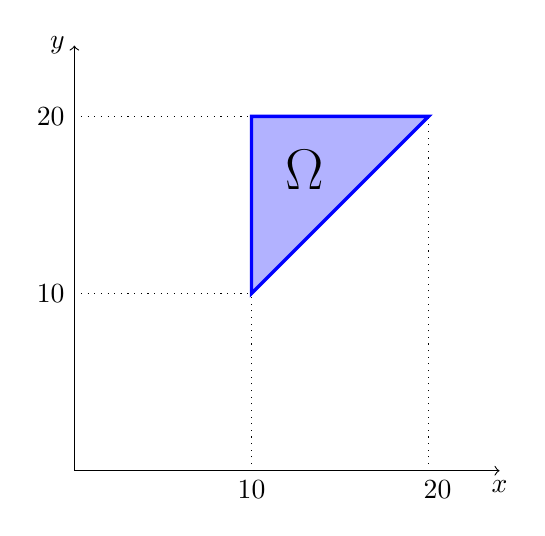
\begin{tikzpicture}[x=0.45cm,y=0.45cm,baseline=(current bounding box.center)]
        \draw[->] (0,0) -- (12,0) node[below] {$x$};
        \draw[->] (0,0) -- (0,12) node[left] {$y$};
        \draw (5,5) -- (10,10) -- (5,10) -- cycle;
        \draw[dotted] (5,0) -- (5,5);
        \draw[dotted] (0,5) -- (5,5);
        \draw[dotted] (10,0) -- (10,10);
        \draw[dotted] (0,10) -- (5,10);
        \node[left] at (0,10) {$20$};
        \node[left] at (0,5) {$10$};
        \node[below] at (10.25,0) {$20$};
        \node[below] at (5,0) {$10$};
        \filldraw[blue, very thick, fill opacity=0.3] (5,5) -- (10,10) -- (5,10) -- cycle;
        \node at (6.5,8.5) {\huge $\Omega$};
    \end{tikzpicture}
    \end{minipage}
    &
    \begin{minipage}{0.45\textwidth}
    \textbf{(a)}\hspace{4pt}
    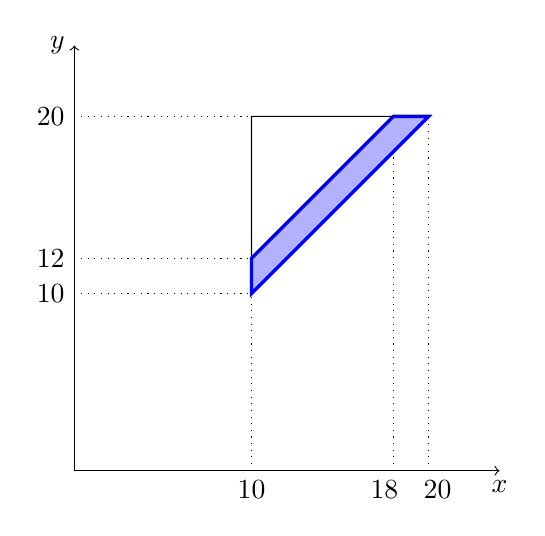
\begin{tikzpicture}[x=0.45cm,y=0.45cm,baseline=(current bounding box.center)]
        \draw[->] (0,0) -- (12,0) node[below] {$x$};
        \draw[->] (0,0) -- (0,12) node[left] {$y$};
        \draw (5,5) -- (10,10) -- (5,10) -- cycle;
        \draw[dotted] (5,0) -- (5,5);
        \draw[dotted] (0,5) -- (5,5);
        \draw[dotted] (10,0) -- (10,10);
        \draw[dotted] (0,10) -- (5,10);
        \node[left] at (0,10) {$20$};
        \node[left] at (0,5) {$10$};
        \node[below] at (10.25,0) {$20$};
        \node[below] at (5,0) {$10$};
        \filldraw[blue, very thick, fill opacity=0.3] (5,5) -- (10,10) -- (9,10) -- (5,6) -- cycle;
        \draw[dotted] (0,6) -- (5,6);
        \draw[dotted] (9,0) -- (9,9);
        \node[left] at (0,6) {$12$};
        \node[below] at (8.75,0) {$18$};
    \end{tikzpicture}
    \end{minipage}
    \\[8mm]
    \begin{minipage}{0.45\textwidth}
    \textbf{(b)}\hspace{4pt}
    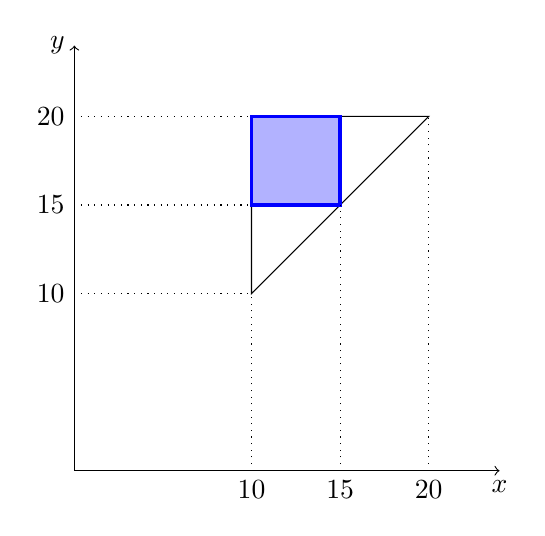
\begin{tikzpicture}[x=0.45cm,y=0.45cm,baseline=(current bounding box.center)]
        \draw[->] (0,0) -- (12,0) node[below] {$x$};
        \draw[->] (0,0) -- (0,12) node[left] {$y$};
        \draw (5,5) -- (10,10) -- (5,10) -- cycle;
        \draw[dotted] (5,0) -- (5,5);
        \draw[dotted] (0,5) -- (5,5);
        \draw[dotted] (10,0) -- (10,10);
        \draw[dotted] (0,10) -- (5,10);
        \node[left] at (0,10) {$20$};
        \node[left] at (0,5) {$10$};
        \node[below] at (10,0) {$20$};
        \node[below] at (5,0) {$10$};
        \filldraw[blue, very thick, fill opacity=0.3] (5,10) -- (7.5,10) -- (7.5,7.5) -- (5,7.5) -- cycle;
        \draw[dotted] (7.5,0) -- (7.5,7.5);
        \draw[dotted] (0,7.5) -- (5,7.5);
        \node[left] at (0,7.5) {$15$};
        \node[below] at (7.5,0) {$15$};
    \end{tikzpicture}
    \end{minipage}
    &
    \begin{minipage}{0.45\textwidth}
    \textbf{(c)}\hspace{4pt}
    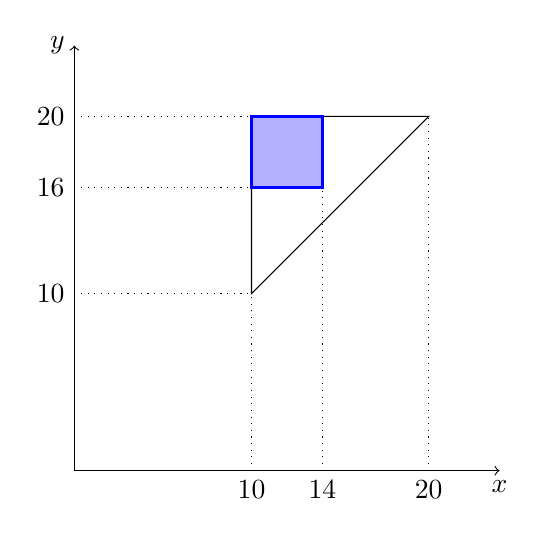
\begin{tikzpicture}[x=0.45cm,y=0.45cm,baseline=(current bounding box.center)]
        \draw[->] (0,0) -- (12,0) node[below] {$x$};
        \draw[->] (0,0) -- (0,12) node[left] {$y$};
        \draw (5,5) -- (10,10) -- (5,10) -- cycle;
        \draw[dotted] (5,0) -- (5,5);
        \draw[dotted] (0,5) -- (5,5);
        \draw[dotted] (10,0) -- (10,10);
        \draw[dotted] (0,10) -- (5,10);
        \node[left] at (0,10) {$20$};
        \node[left] at (0,5) {$10$};
        \node[below] at (10,0) {$20$};
        \node[below] at (5,0) {$10$};
        \filldraw[blue, very thick, fill opacity=0.3] (5,10) -- (7,10) -- (7,8) -- (5,8) -- cycle;
        \draw[dotted] (7,0) -- (7,8);
        \draw[dotted] (0,8) -- (5,8);
        \node[left] at (0,8) {$16$};
        \node[below] at (7,0) {$14$};
    \end{tikzpicture}
    \end{minipage}
    \\[8mm]
    \begin{minipage}{0.45\textwidth}
    \textbf{(d)}\hspace{4pt}
    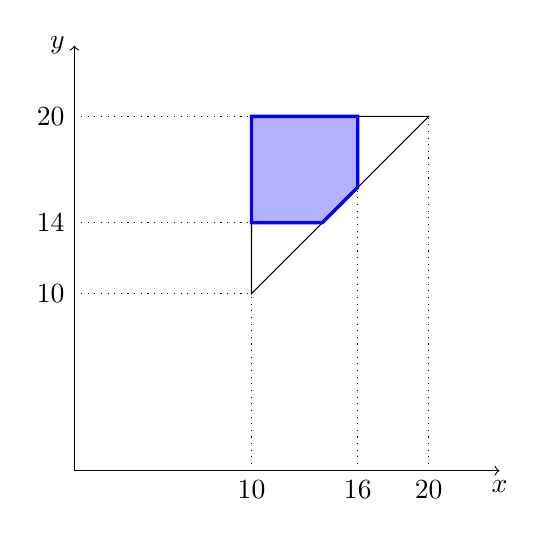
\begin{tikzpicture}[x=0.45cm,y=0.45cm,baseline=(current bounding box.center)]
        \draw[->] (0,0) -- (12,0) node[below] {$x$};
        \draw[->] (0,0) -- (0,12) node[left] {$y$};
        \draw (5,5) -- (10,10) -- (5,10) -- cycle;
        \draw[dotted] (5,0) -- (5,5);
        \draw[dotted] (0,5) -- (5,5);
        \draw[dotted] (10,0) -- (10,10);
        \draw[dotted] (0,10) -- (5,10);
        \node[left] at (0,10) {$20$};
        \node[left] at (0,5) {$10$};
        \node[below] at (10,0) {$20$};
        \node[below] at (5,0) {$10$};
        \filldraw[blue, very thick, fill opacity=0.3] (5,10) -- (8,10) -- (8,8) -- (7,7) -- (5,7) -- cycle;
        \draw[dotted] (8,0) -- (8,8);
        \draw[dotted] (0,7) -- (5,7);
        \node[left] at (0,7) {$14$};
        \node[below] at (8,0) {$16$};
    \end{tikzpicture}
    \end{minipage}
    &
    \begin{minipage}{0.45\textwidth}
    \textbf{(e)}\hspace{4pt}
    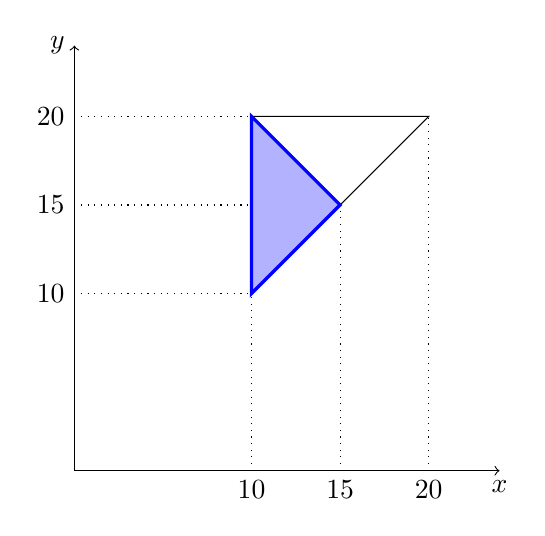
\begin{tikzpicture}[x=0.45cm,y=0.45cm,baseline=(current bounding box.center)]
        \draw[->] (0,0) -- (12,0) node[below] {$x$};
        \draw[->] (0,0) -- (0,12) node[left] {$y$};
        \draw (5,5) -- (10,10) -- (5,10) -- cycle;
        \draw[dotted] (5,0) -- (5,5);
        \draw[dotted] (0,5) -- (5,5);
        \draw[dotted] (10,0) -- (10,10);
        \draw[dotted] (0,10) -- (5,10);
        \node[left] at (0,10) {$20$};
        \node[left] at (0,5) {$10$};
        \node[below] at (10,0) {$20$};
        \node[below] at (5,0) {$10$};
        \filldraw[blue, very thick, fill opacity=0.3] (5,5) -- (7.5,7.5) -- (5,10) -- cycle;
        \draw[dotted] (7.5,0) -- (7.5,7.5);
        \draw[dotted] (0,7.5) -- (5,7.5);
        \node[left] at (0,7.5) {$15$};
        \node[below] at (7.5,0) {$15$};
    \end{tikzpicture}
    \end{minipage}
    \end{tabular}
    \end{center}
    (try to find mathematical justifications for these shapes).
\end{sol}

\begin{sol}{complement-probability}
    We have already established finite additivity in Problem~\ref{prob:finiteadd}, which impllies that
    \[
        \PP(A)+\PP(\overline{A})=\PP(A\cup\overline{A})=\PP(\Omega)=1,
    \]
    hence $\PP(\overline{A})=1-\PP(A)$.
\end{sol}

\begin{sol}{shootingthreetimes}
    \begin{enumerate}
        \item[(a)] $\PP(\text{3 hits}) = \PP(A_1\cap A_2\cap A_3) = P_1P_2P_3$.
        \item[(b)] $\PP(\text{2 hits}) = \PP(A_1\cap A_2\cap\overline{A_3}) + \PP(A_1\cap\overline{A_2}\cap A_3) + \PP(\overline{A_1}\cap A_2\cap A_3) = \\
        \hphantom{\PP(\text{2 hits})} = P_1P_2(1-P_3) + P_1(1-P_2)P_3 + (1-P_1)P_2P_3$.
        \item[(c)] $\PP(\text{at least 2 hits}) = \PP(\text{3 hits}) + \PP(\text{2 hits}) = \\
        \hphantom{\PP(\text{at least 2 hits})} = P_1P_2P_3 + P_1P_2(1-P_3) + P_1(1-P_2)P_3 + (1-P_1)P_2P_3$.
        \item[(d)] $\PP(\text{0 hits}) = \PP(\overline{A_1}\cap\overline{A_2}\cap\overline{A_3})=(1-P_1)(1-P_2)(1-P_3)$.
        \item[(e)] $\PP(\text{at lease 1 hit})=1-\PP(\text{0 hits})=1-(1-P_1)(1-P_2)(1-P_3)$.
        \item[(f)] $\PP(\text{even hits})=\PP(\text{0 hits})+\PP(\text{2 hits})=\\
        \hphantom{\PP(\text{even hits})}=(1-P_1)(1-P_2)(1-P_3)+P_1P_2(1-P_3) + P_1(1-P_2)P_3 + (1-P_1)P_2P_3$.
        \item[(g)] $\PP(\text{odd hits})=\PP(\text{1 hit})+\PP(\text{3 hits})=\\
        \hphantom{\PP(\text{odd hits})}=P_1(1-P_2)(1-P_3)+(1-P_1)P_2(1-P_3)+(1-P_1)(1-P_2)P_3+P_1P_2P_3$.
    \end{enumerate}
\end{sol}

\begin{sol}{geom1}
    The events $A$, $B$, $A\cup B$, $A\cap B$, $A\setminus B$, $\overline{A}\cup\overline{B}$ are shown below.
    Note that the condition $x+y\le1$ is equivalent to $y\le1-x$, hence $A$ is the region under the curve $y=1-x$, and $B$ is the region under $y=x^2$.
    \begin{center}
    \begin{tabular}{ccc}
    
    \begin{minipage}{0.3\textwidth}
    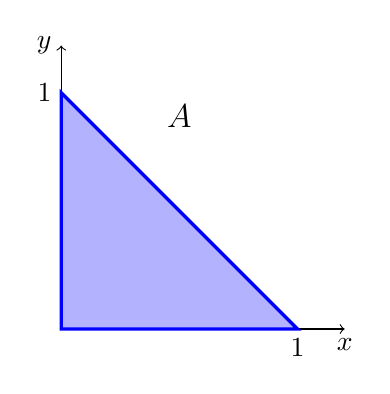
\begin{tikzpicture}[x=0.3cm,y=0.3cm,baseline=(current bounding box.center)]
        \draw[->] (0,0) -- (12,0) node[below] {$x$};
        \draw[->] (0,0) -- (0,12) node[left] {$y$};
        \node[left] at (0,10) {$1$};
        \node[below] at (10,0) {$1$};
        \filldraw[blue, very thick, fill opacity=0.3]
            (0,0) -- (10,0) -- (0,10) -- cycle;
        \node at (5,9) {\large $A$};
    \end{tikzpicture}
    \end{minipage}
    &
    \begin{minipage}{0.3\textwidth}
    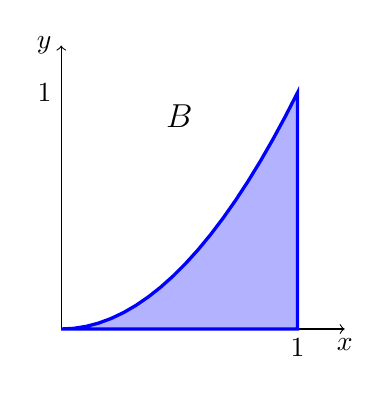
\begin{tikzpicture}[x=0.3cm,y=0.3cm,baseline=(current bounding box.center)]
        \draw[->] (0,0) -- (12,0) node[below] {$x$};
        \draw[->] (0,0) -- (0,12) node[left] {$y$};
        \node[left] at (0,10) {$1$};
        \node[below] at (10,0) {$1$};
        \filldraw[blue, very thick, fill opacity=0.3, samples=20, domain=0:10]
            plot (\x, {\x*\x/10}) -- (10,0) -- (0,0) -- cycle;
        \node at (5,9) {\large $B$};
    \end{tikzpicture}
    \end{minipage}
    &
    \begin{minipage}{0.3\textwidth}
    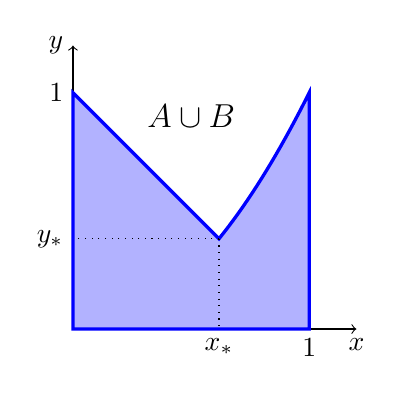
\begin{tikzpicture}[x=0.3cm,y=0.3cm,baseline=(current bounding box.center)]
        \draw[->] (0,0) -- (12,0) node[below] {$x$};
        \draw[->] (0,0) -- (0,12) node[left] {$y$};
        \node[left] at (0,10) {$1$};
        \node[below] at (10,0) {$1$};
        \pgfmathsetmacro\xa{-5 + 5*sqrt(5)}
        \filldraw[blue, very thick, fill opacity=0.3, samples=20]
            (0,0) -- (10,0) -- plot[domain=10:\xa] (\x, {\x*\x/10}) -- plot[domain=\xa:0] (\x, {10-\x}) -- cycle;
        \node at (5,9) {\large $A\cup B$};
        \pgfmathsetmacro\ya{10 - \xa}
        \draw[dotted] (\xa,\ya) -- (\xa,0);
        \draw[dotted] (\xa,\ya) -- (0,\ya);
        \node[left] at (0,\ya) {$y_*$};
        \node[below] at (\xa,0) {$x_*$};
    \end{tikzpicture}
    \end{minipage}
    \\[8mm]
    \begin{minipage}{0.3\textwidth}
    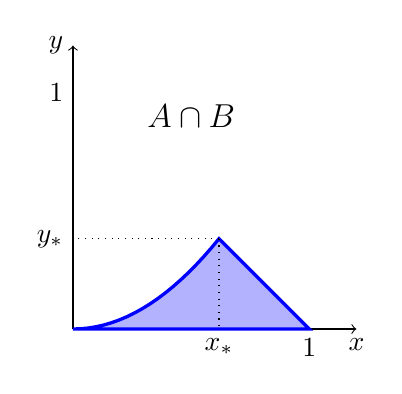
\begin{tikzpicture}[x=0.3cm,y=0.3cm,baseline=(current bounding box.center)]
        \draw[->] (0,0) -- (12,0) node[below] {$x$};
        \draw[->] (0,0) -- (0,12) node[left] {$y$};
        \node[left] at (0,10) {$1$};
        \node[below] at (10,0) {$1$};
        \pgfmathsetmacro\xa{-5 + 5*sqrt(5)}
        \filldraw[blue, very thick, fill opacity=0.3, samples=20, domain=0:\xa]
            (0,0) -- plot (\x, {\x*\x/10}) -- (10,0) -- cycle;
        \node at (5,9) {\large $A\cap B$};
        \pgfmathsetmacro\ya{10 - \xa}
        \draw[dotted] (\xa,\ya) -- (\xa,0);
        \draw[dotted] (\xa,\ya) -- (0,\ya);
        \node[left] at (0,\ya) {$y_*$};
        \node[below] at (\xa,0) {$x_*$};
    \end{tikzpicture}
    \end{minipage}
    &
    \begin{minipage}{0.3\textwidth}
    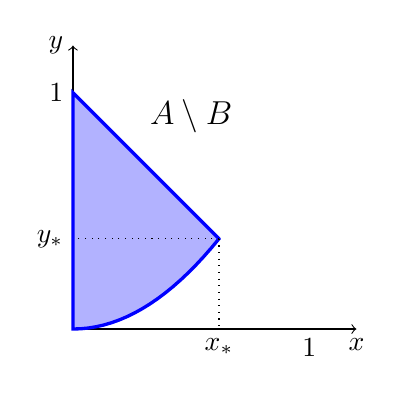
\begin{tikzpicture}[x=0.3cm,y=0.3cm,baseline=(current bounding box.center)]
        \draw[->] (0,0) -- (12,0) node[below] {$x$};
        \draw[->] (0,0) -- (0,12) node[left] {$y$};
        \node[left] at (0,10) {$1$};
        \node[below] at (10,0) {$1$};
        \pgfmathsetmacro\xa{-5 + 5*sqrt(5)}
        \filldraw[blue, very thick, fill opacity=0.3, samples=20]
            (0,10) -- plot[domain=0:\xa] (\x, {10-\x}) -- plot[domain=\xa:0] (\x, {\x*\x/10}) -- cycle;
        \node at (5,9) {\large $A\setminus B$};
        \pgfmathsetmacro\ya{10 - \xa}
        \draw[dotted] (\xa,\ya) -- (\xa,0);
        \draw[dotted] (\xa,\ya) -- (0,\ya);
        \node[left] at (0,\ya) {$y_*$};
        \node[below] at (\xa,0) {$x_*$};
    \end{tikzpicture}
    \end{minipage}
    &
    \begin{minipage}{0.3\textwidth}
    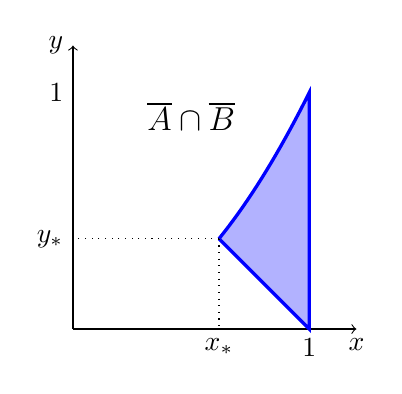
\begin{tikzpicture}[x=0.3cm,y=0.3cm,baseline=(current bounding box.center)]
        \draw[->] (0,0) -- (12,0) node[below] {$x$};
        \draw[->] (0,0) -- (0,12) node[left] {$y$};
        \node[left] at (0,10) {$1$};
        \node[below] at (10,0) {$1$};
        \pgfmathsetmacro\xa{-5 + 5*sqrt(5)}
        \filldraw[blue, very thick, fill opacity=0.3, samples=20]
            (10,0) -- plot[domain=10:\xa] (\x, {10-\x}) -- plot[domain=\xa:10] (\x, {\x*\x/10}) -- (10,0) -- cycle;
        \node at (5,9) {\large $\overline{A}\cap\overline{B}$};
        \pgfmathsetmacro\ya{10 - \xa}
        \draw[dotted] (\xa,\ya) -- (\xa,0);
        \draw[dotted] (\xa,\ya) -- (0,\ya);
        \node[left] at (0,\ya) {$y_*$};
        \node[below] at (\xa,0) {$x_*$};
    \end{tikzpicture}
    \end{minipage}
    \end{tabular}
    \end{center}
    To draw $A\cup B$, $A\cap B$, $A\setminus B$, and $\overline{A}\cap\overline{B}$ we need to find the intersection point $(x_*,y_*)$ of the graphs of $y=1-x$ and $y=x^2$. For that purpose we set $x^2=1-x$, and solve for $x$ to get $x=\frac{-1\pm\sqrt5}{2}$. We need the one between $0$ and $1$, hence $x_*=\frac{\sqrt5-1}{2}$. Plugging in either one of the equations we get $y_*=\frac{3-\sqrt5}{2}$ Hence the intersection point is $(\frac{\sqrt5-1}{2},\frac{3-\sqrt5}{2})$.
    \[
        \PP(A) = \frac{|A|}{|\Omega|}=|A|=\int_0^11-x\,dx=\frac12,
    \]
    \[
        \PP(B) = \frac{|B|}{|\Omega|}=|B|=\int_0^1x^2\,dx=\left[\frac{x^3}{3}\right]_0^1=\frac13-0=\frac13,
    \]
    \begin{align*}
        \PP(A\cup B) &= \int_0^{x_*}1-x\,dx + \int_{x_*}^1x^2\,dx
        = \left[x-\frac{x^2}{2}\right]_0^{x_*}+\left[\frac{x^3}{3}\right]_{x_*}^1
        = x_*-\frac{x_*^2}{2}+\frac{1}{3}-\frac{x_*^3}{3} \\
        &=x_*-\frac{1-x_*}{2}+\frac{1}{3}-\frac{2x_*-1}{3}
        = \frac{3x_*-1}{2}+\frac{2(1-x_*)}{3} = \frac{5x_*+1}{6} \\
        &= \frac{5\cdot\frac{\sqrt5-1}{2}+1}{6} = \frac{5\sqrt{5}-3}{12},
    \end{align*}
    \[
        \PP(A\cap B)=\PP(A)+\PP(B)-\PP(A\cup B)=\frac12+\frac13-\frac{5\sqrt{5}-3}{12}=\frac{13-5\sqrt5}{12},
    \]
    \[
        \PP(A\setminus B)=\PP(A)-\PP(A\cap B)=\frac12-\frac{13-5\sqrt5}{12}=\frac{6-(13-5\sqrt5)}{12}=\frac{5\sqrt5-7}{12},
    \]
    \[
        \PP(\overline{A}\cap\overline{B})=\PP(\overline{A\cup B})=1-\PP(A\cup B)=1-\frac{5\sqrt5-3}{12}=\frac{15-5\sqrt5}{12}.
    \]
\end{sol}

\begin{sol}{polynom1}
    Let $\Omega=\{1,2,\ldots,6\} ^3$. There are $6^3=216$ outcomes in $\Omega$.
    \begin{enumerate}
        \item[(a)] Let $A$ be the event of the roots being real. Then $\{(a,b,c)\in\Omega\mid b^2-4ac\ge0$\}. The condition $b^2-4ac\ge0$ is equivalent to $ac\le\frac{b^2}{4}$. Note that $\frac{b^2}{4}$ is at most $9$, therefore so is $ac$. Now we list the number of $(a,c)$ pairs for which $ac=k$, where $1\le k\le9$:
        \begin{align*}
            ac=1\quad&:\quad\text{1 pair}:\quad(1,1),\\
            ac=2\quad&:\quad\text{2 pairs}:\quad(1,2),(2,1),\\
            ac=3\quad&:\quad\text{2 pairs}:\quad(1,3),(3,1),\\
            ac=4\quad&:\quad\text{3 pairs}:\quad(1,4),(2,2),(4,1),\\
            ac=5\quad&:\quad\text{2 pairs}:\quad(1,5),(5,1),\\
            ac=6\quad&:\quad\text{4 pairs}:\quad(1,6),(2,3),(3,2),(6,1),\\
            ac=7\quad&:\quad\text{0 pairs},\\
            ac=8\quad&:\quad\text{2 pairs}:\quad(2,4),(4,2),\\
            ac=9\quad&:\quad\text{1 pair}:\quad(3,3).
        \end{align*}
        Then for each value of $b$ we can count how many of these pairs satisfy $ac\le\frac{b^2}{4}$.
        \begin{align*}
            &b=1\quad\Longrightarrow\quad\left\lfloor b^2/4\right\rfloor=0
            \quad\Longrightarrow\quad 0\\
            &b=2\quad\Longrightarrow\quad\left\lfloor b^2/4\right\rfloor=1
            \quad\Longrightarrow\quad 1\\
            &b=3\quad\Longrightarrow\quad\left\lfloor b^2/4\right\rfloor=2
            \quad\Longrightarrow\quad 1+2=3\\
            &b=4\quad\Longrightarrow\quad\left\lfloor b^2/4\right\rfloor=4
            \quad\Longrightarrow\quad 1+2+2+3=8\\
            &b=5\quad\Longrightarrow\quad\left\lfloor b^2/4\right\rfloor=6
            \quad\Longrightarrow\quad 1+2+2+3+2+4=14\\
            &b=6\quad\Longrightarrow\quad\left\lfloor b^2/4\right\rfloor=9
            \quad\Longrightarrow\quad 1+2+2+3+2+4+2+1=17
        \end{align*}
        The number of favorable outcomes is $1+3+8+14+17=43$, so $\PP(A)=\frac{43}{216}\approx0.2$.
        \item[(b)] The roots are rational if and only if $b^2-4ac$ is a perfect square. Considering the fact that $b^2-4ac\le b^2\le6^2=36$ we conclude that the only possible values are $0$, $1$, $4$, $9$, $16$, and $25$. Note that $b^2-4ac=k^2$ is equivalent to $ac=\frac{b^2-k^2}{4}$, so we can list the cases where $\frac{b^2-k^2}{4}$ is an integer and can be written as a product of $a$ and $c$:
        \[
        \begin{array}{c|c|c|c}
            b & k & \frac{b^2-k^2}{4} & \#(a,c) \\
            \hline
            2 & 0 & 1 & 1 \\
            3 & 1 & 2 & 2 \\
            4 & 0 & 4 & 3 \\
            4 & 2 & 3 & 2 \\
            5 & 1 & 6 & 4 \\
            5 & 3 & 4 & 3 \\
            6 & 0 & 9 & 1 \\
            6 & 2 & 8 & 2 \\
            6 & 4 & 5 & 2
        \end{array}
        \]
        The last column shows the number of pairs $(a,c)$ such that $ac=\frac{b^2-k^2}{4}$.
        \[
            \PP(\text{rational roots})=\frac{1+2+3+2+4+3+1+2+2}{216}=\frac{20}{216}=\frac{5}{54}.
        \]
    \end{enumerate}
\end{sol}

\begin{sol}{inclusion-exclusion-simple}
    Observe that $A=(A\setminus B)\cup(A\cap B)$, with $A\setminus B$ and $A\cap B$ being disjoint. The same holds for $B=(B\setminus A)\cup(A\cap B)$, with $B\setminus A$ and $A\cap B$ being disjoint. This allows us to write
    \[
        \PP(A)=\PP(A\setminus B)+\PP(A\cap B),\qquad\PP(B)=\PP(B\setminus A)+\PP(A\cap B).
    \]
    Noting that $A\cup B=(A\setminus B)\cup(B\setminus A)\cup(A\cap B)$ and combining the two equations above we get
    \[
        \PP(A)+\PP(B)=\PP(A\setminus B)+\PP(A\cap B)+\PP(B\setminus A)+\PP(A\cap B)=\PP(A\cup B)+\PP(A\cap B).
    \]
\end{sol}

\begin{sol}{weirdlimit}
    Obviously, there are exactly $\left\lfloor\frac{n}{k}\right\rfloor$ numbers in $\{1,2,\ldots,n\}$ that are divisible by $k$ (which are $k, 2k, \ldots, \left\lfloor n/k\right\rfloor k$). Therefore
    \[
        p_n=\frac{\left\lfloor n/k\right\rfloor}{n}.
    \]
    For the limit, write $n=qk+r$ with $0\le r<k$. Then $\lfloor n/k\rfloor=q$, so
    \[
        p_n=\frac{q}{qk+r}=\frac{1}{k+r/q}\longrightarrow\frac{1}{k}.
    \]
\end{sol}

\begin{sol}{unit-circle-square}
    \[
    \PP(\text{point in square})=\frac{\text{area of square}}{\text{area of circle}}=\frac2\pi.
    \]
\end{sol}

\begin{sol}{geometric2d}
    \begin{minipage}{0.69\textwidth}
    In the geometric probability model the sample space is the square $\Omega=[0,1]^2$. We choose a random point $(x,y)$ and calculate $|x-y|$. The probability that $|x-y|<\alpha$ is the area of the region satisfying this condition, which can be split into the conditions $x-y<\alpha$ and $x-y>-\alpha$. The corresponding region $A$ for the case $\alpha=0.3$ is shown in the picture. The probability is therefore
    \end{minipage}
    \hfill
    \begin{minipage}{0.3\textwidth}
    \centering
    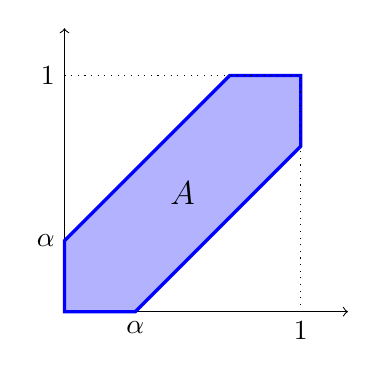
\begin{tikzpicture}[x=0.3cm,y=0.3cm,baseline=(current bounding box.center)]
        \draw[->] (0,0) -- (12,0);
        \draw[->] (0,0) -- (0,12);
        \node[left] at (0,10) {$1$};
        \node[below] at (10,0) {$1$};
        \filldraw[blue, very thick, fill opacity=0.3]
            (0,0) -- (3,0) -- (10,7) -- (10,10) -- (7,10) -- (0,3) -- cycle;
        \node at (5,5) {\large $A$};
        \draw[dotted] (10,0) -- (10,10);
        \draw[dotted] (0,10) -- (10,10);
        \node[left] at (0,3) {$\alpha$};
        \node[below] at (3,0) {$\alpha$};
    \end{tikzpicture}
    \end{minipage}
    \[
        \PP(A)=1-\PP(\overline{A})=1-(1-\alpha)^2=1-1+2\alpha-\alpha^2=2\alpha-\alpha^2=(2-\alpha)\alpha.
    \]
\end{sol}